\section{ Solving probleme by search}
\subsection{Structure d'un agent}
	Un agent est composé de 2 partie :
	\begin{itemize}
		\item \textbf{Architecture} : c'est les composants de l'ordinateur sur le quelle l'agent tourne
		\item \textbf{Programme} : Se sont les fonctions qui Map les perceptions en actions
	\end{itemize}
	
	Exemple d'un programme d'agent:
	
	\begin{itemize}
		\item Table de conduite de l'agent (\textbf{table driven})\\
		\item une table essor : Tous les states atteignable depuis le state actuelle\\
		\item \textbf{Path} : Séquence de states connecté par une sequence d'action\\
		\item \textbf{Operators} : Manière de modifier un state avec une action\\
		\item \textbf{Goals Test} : Fonction qui teste si un state est le résultat final\\
		\item \textbf{Step Cost} : Cout numérique de passer du state $s$ avec l'action $a$ pour passer au state $s'$\\
		\item \textbf{Path Cost} : Fonction qui donne un cout a chaque path\\
		\item \textbf{Solution} : Séquence d'action de l'initial state jusqu'au goal state\\
		\item \textbf{Optimal Solution} : Solution avec le path avec le plus petit cout parmi toutes les solutions\\
		\item \textbf{Node} : Data structure qui constitue les graph et arbre de recherche\\
		\item \textbf{Frontier} : Ensemble de Node généré au quelle les ancêtre on été Goal-tested (visited)\\
		
		\item \textit{C'étais long mais bon fallait le faire}
		
	\end{itemize}
	\subsection{Problem solving Agent}
		\subsubsection{Definition Probleme}
			Un problème peut être définie avec :
			\begin{enumerate}
				\item States ou Initial State
				\item Une description des actions possible et valide par l'agent
				\item Une description de quoi chaque action fait (transition model)
				\item Un Goal test
				\item Un Path cost qui utilise un step cost
			\end{enumerate}
		\subsubsection{Solution}
			Une solution est une séquence d'action qui commence du state initial et qui termine à un des goal state. La solution est optimal si elle a la plus petite path cost parmis toutes les solutions
		\subsubsection{State space}
			Ensemble qui représente le problème avec les actions, les couts, ... (graph représentation). Possibilité d'un ensemble infini de states.
			\begin{figure}[htp]
				\centering
				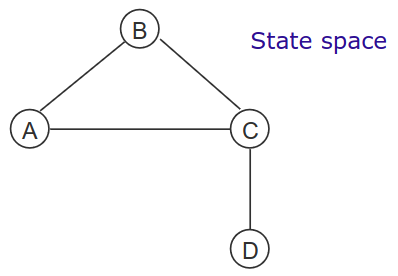
\includegraphics[width=.5\textwidth]{img/StateSpace.png}
			\end{figure}
		\subsubsection{Search Tree}
			Représentation du problème sous la forme d'arbre, avec les path entre les states et les goals. multiple path. Et un seul path d'un node a la racine.
			\begin{figure}[htp]
				\centering
				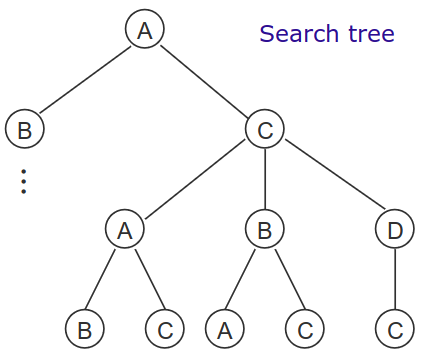
\includegraphics[width=.5\textwidth]{img/SearchTree.png}
			\end{figure}
			
		\subsubsection{State and Nodes}
			\begin{itemize}
				\item \textbf{State} représentation d'un configuration physique qui represente un state intermédiaire.
				\item \textbf{Node} data structure qui constitue le search tree
			\end{itemize}
			il peut y avoir plusieurs nodes avec le même state
		\subsubsection{Repeated States}
			On va éviter de visiter des Nodes qui on déjà été visité avant, pour cela, on va utiliser la représentation en arbre (search tree) et on ne pas va \textit{Expand} les nodes déjà visité.
	\subsection{Searching for Solutions}
		Trouver une solution est le fait de traverser un state space (graph ou tree) et du initial state au goal state avec un ensemble d'actions valide.


		\textbf{Expanding} : appliquer chaque action légal au state actuel.
		\begin{figure}[htp]
			\centering
			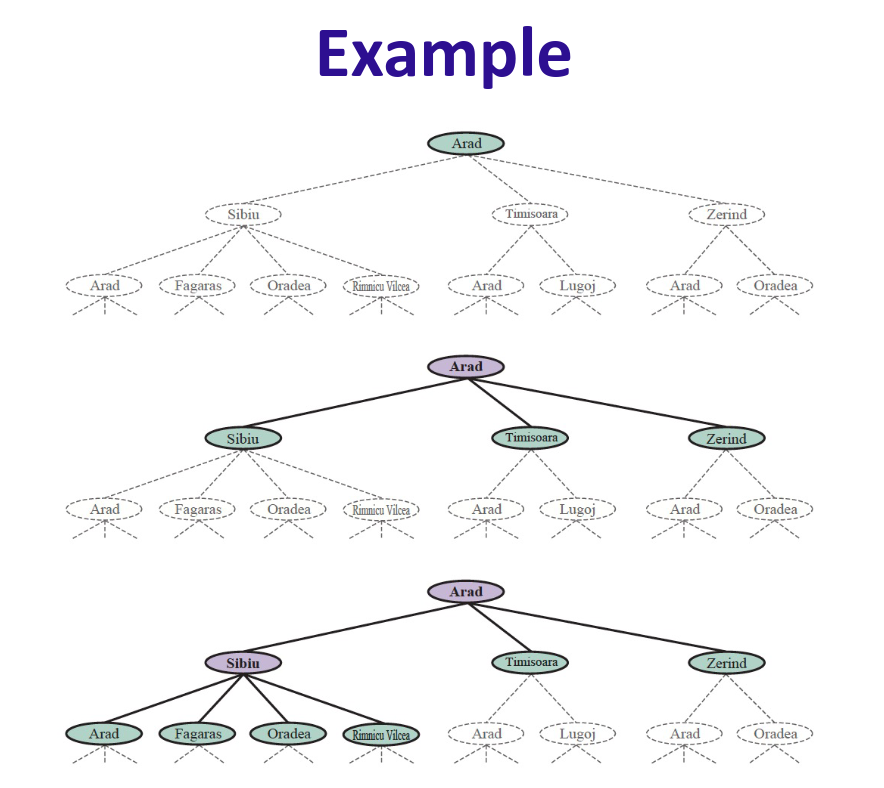
\includegraphics[width=0.6\textwidth]{img/ExempleExpanding.png}
		\end{figure}
		
		\textbf{Frontier} : Ensemble des node non-Expanded au quelle les ancêtres on déjà été visité. La frontière peut être représenté grâce a une Data structure Queue (lol zizi), On peut utiliser un Priority, LIFO, FIFO, \dots
		\begin{figure}[htp]
			\centering
			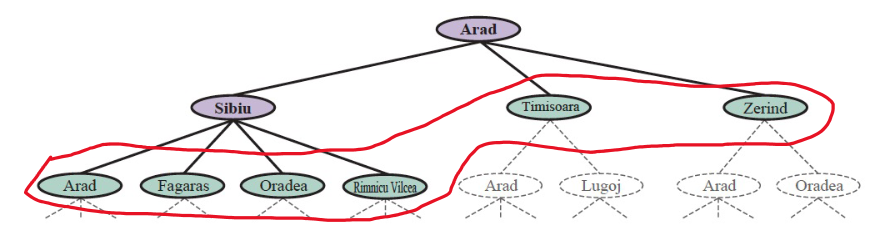
\includegraphics[width=0.6\textwidth]{img/FrontierExemple.png}
		\end{figure}
		
		\subsubsection{Stratégies}
			Il y a 2 types de recherches: 
			\begin{enumerate}
				\item \textbf{uninformed search} où la seul information de l'agent est \textit{"suis-je le but final ?"}.
				\item \textbf{informed search} où l'agent a les informations d'avant.
			\end{enumerate}
			
			On peut évaluer ces recherche avec 4 critères:
			\begin{itemize}
				\item \textbf{Completeness} : l'agent trouve un solution s'il en existe au moins une.
				\item \textbf{Time complexity} : Souvent en terme du nombre de nodes généré/Expanded
				\item \textbf{Space complexity} : Nombre de node en mémoire
				\item \textbf{Optimality} : Trouve solution avec le cout minimal 
			\end{itemize}
			
			On va utiliser 3 variables :
			\begin{itemize}
				\item \textbf{b} : Facteur de branchement maximal du Search tree
				\item \textbf{d} : Profondeur de la solution la moins couteuse
				\item \textbf{m} : Profondeur max de l'arbre (peut etre $\infty$)
			\end{itemize}
	\subsection{Uninformed Search}
		\begin{figure}[htp]
			\centering
			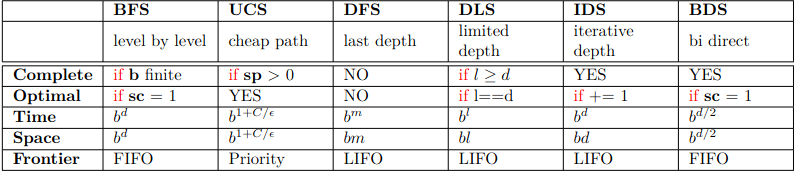
\includegraphics[width=\textwidth]{img/UninformedSearch.png}
		\end{figure}
		\subsubsection{Breadth-First Search(BFS)}
			Le but est de vérifier par niveau de l'arbre. Problème la mémoire est vite remplie. On commence du root node et ensuite on passe au sub-nodes qui sont dans une FIFO Queue qui représente la frontière.
			
			Il est \textbf{complet} si $b$ est fini, il est \textbf{Optimal} si le cout part étapes est de $1$ (souvent il n'est pas optimal)
			
			La complexité temporelle et de $\mathcal{O}(b^d)$ \footnote{$1+b+b^2 + \dots + b^d + b(b^d - 1) = \mathcal{O}(b^{d+2}) = \mathcal{O}(b^d)$} et la complexité spatial est de $\mathcal{O}(b^d)$	
			
			\begin{figure}[htp]
				\centering
				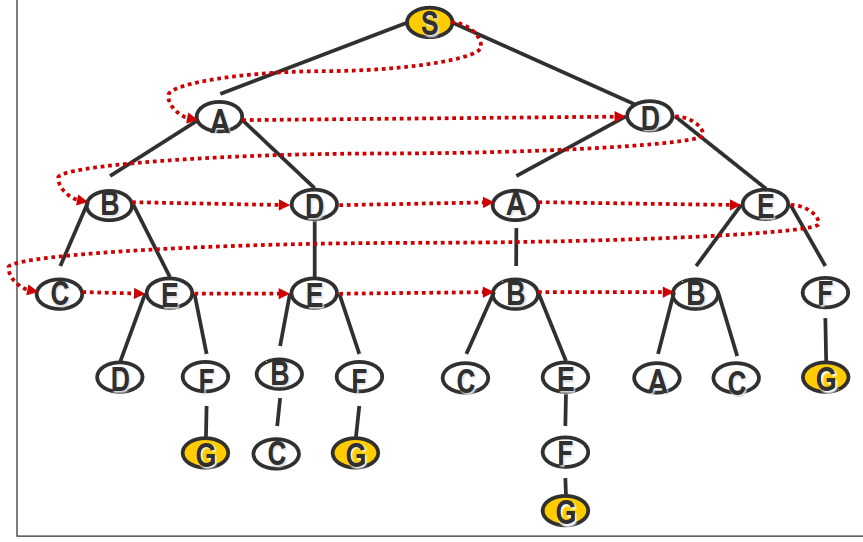
\includegraphics[width=0.6\textwidth]{img/BFS.png}
				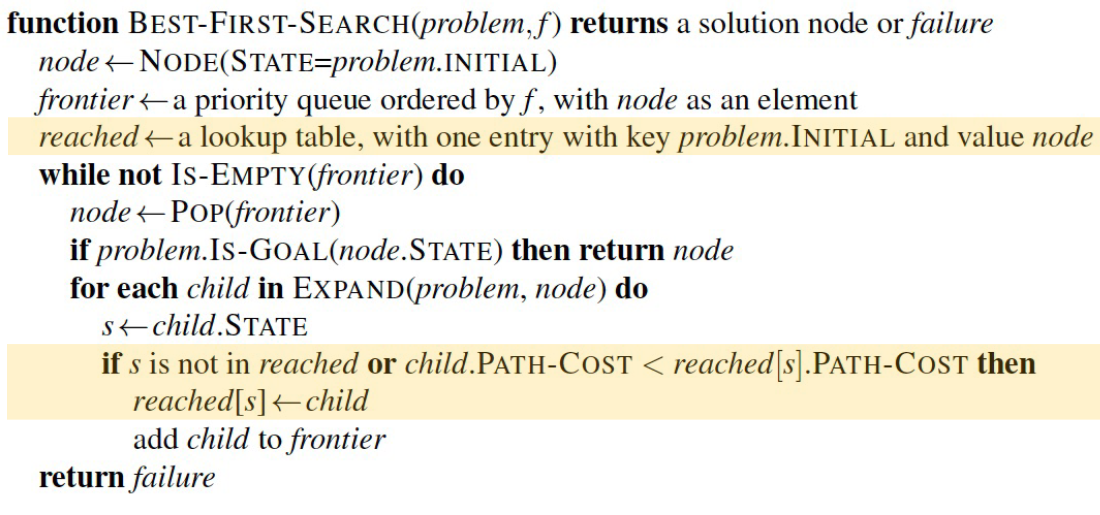
\includegraphics[width=\textwidth]{img/CodeBFS.png}
			\end{figure}					
		\newpage
		\subsubsection{Uniform-Cost search (UCS)}
			Comme le BFS sauf que le Node avec le cout le plus petit est exploré en premier. Il y a un cout pour passer d'un node a l'autre. La frontière est implémenté avec un Priorety Queue.
			
			\begin{figure}[htp]
				\centering
				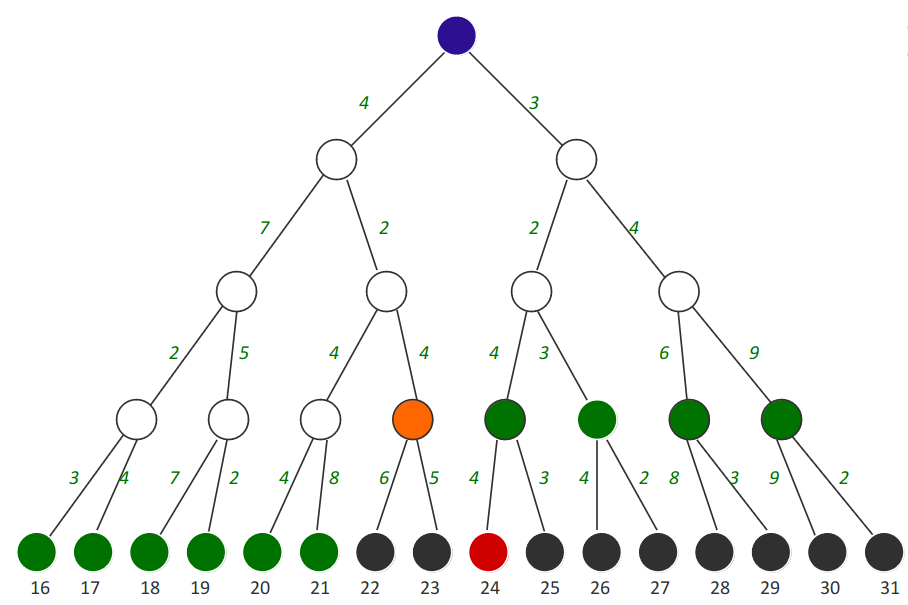
\includegraphics[width=0.6\textwidth]{img/UCS.png}
			\end{figure}
			
			L'algo est \textbf{Complet} si le cout entre chaque step est strictement positif ($\geq \epsilon$), \textbf{Time et Space complexity} = $\mathcal{O}(b^{C^{*}/\epsilon})$	ou $C^*$ est le cout optimal de la solution, et il est \textbf{Optimal} car les node sont expanded par ordre croissant grâce à la Priority Queue.
			
		\subsubsection{Depth-first Search (DFS)}
		Concrètement, on visite toutes une branche de l'arbre jusqu'à arriver à la \textit{Leaf}, si on ne trouve pas le goal on passe a la prochaine, etc.
		La Frontière est implémenté avec un Queue LIFO.
		
		Cette algo n'est pas \textbf{Complete} car il peut tomber dans une boucle infinie, la \textbf{Complexity time} est de $\mathcal{O}(b^m)$ et la \textbf{Space complexity} est de $\mathcal{O}(mb)$, \textbf{Il n'est pas optimal}
		
		\begin{figure}[htp]
			\centering
			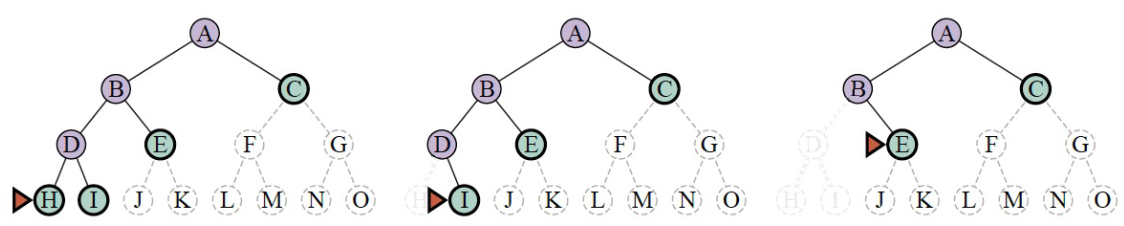
\includegraphics[width=\textwidth]{img/ExempleDFS.png}
		\end{figure}
		
		\subsubsection{Depth-Limited Search}
			Pareil de DFS sauf que la on met une limite de profondeur(depth) $l$.
		
		\subsubsection{Iterative Deepening}		
		  Pareil que DLS mais si $l < d$ alors on ne trouveras jamais de solutions, donc on va incrémenter petit a petit $l$
			\begin{figure}[htp]
				\centering
				$l = 1$
				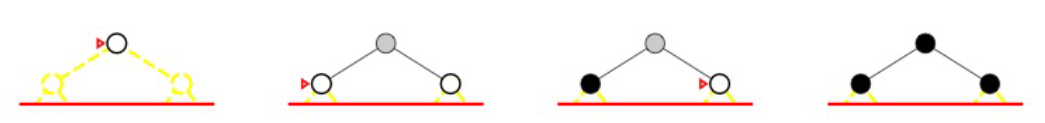
\includegraphics[width=\textwidth]{img/DLS1.png}
				$l = 2$
				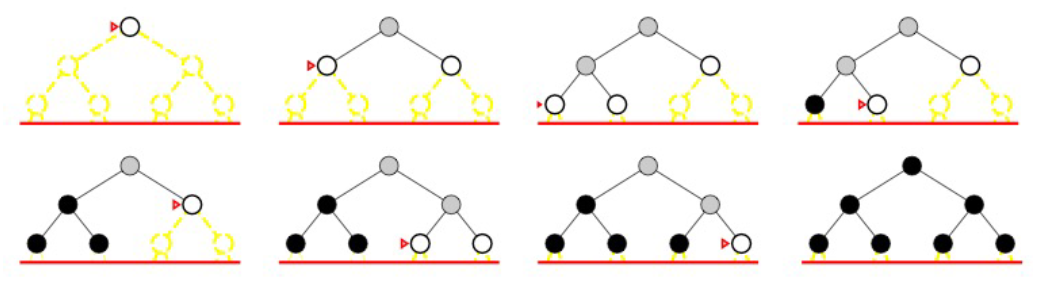
\includegraphics[width=\textwidth]{img/DLS2.png}
				$l = 3$
				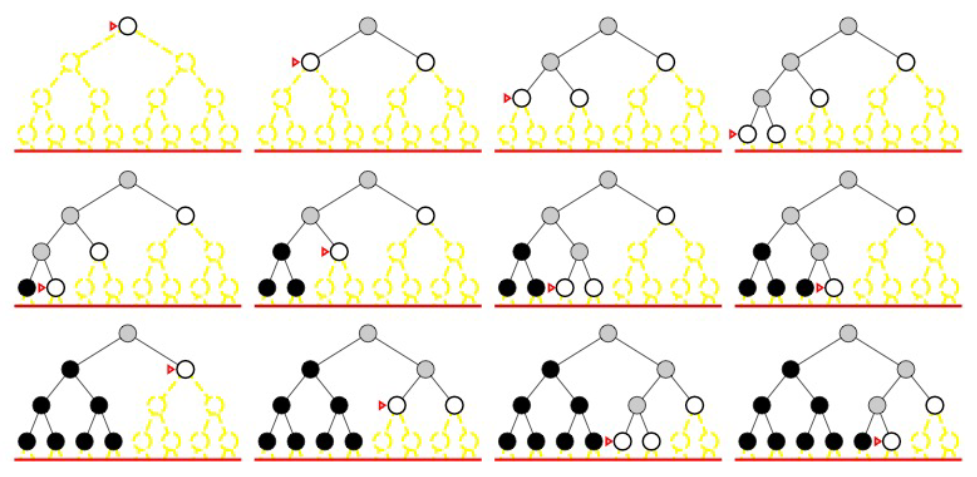
\includegraphics[width=\textwidth]{img/DLS3.png}

			\end{figure}
			
		Plusieurs nodes sont visité plusieurs fois, mais ce n'est pas très grave car il n'y en a pas beaucoup.
		
		Cet algo est \textbf{Complete} et \textbf{Optimal} si on incrémente de 1 à 1
		
		la \textbf{Complexité temporel} est $\mathcal{O}(b^d)$ et la \textbf{Space complexity} est $\mathcal{O}(bd)$
		
		
		\subsubsection{Biderectional Search}
			On commence du root jusqu'au Goal et aussi du Goal jusqu'au root et on stoppe quand les 2 s'intersecte. Il y quelque difficulté.
			\begin{itemize}
				\item Prédécesseurs du goal doivent être généré (pas toujours possible)
				\item Search doit être coordonnée entre les 2 recherches
				\item Problème si plusieurs Goal
				\item Tous les nodes doivent rester en mémoire
			\end{itemize}
			
	\subsection{Informed Search}
		En utilisant des connaissances spécifiques au problème, trouver et/ou déduire des informations sur les States futurs et les paths futures.
		
		BFS est un algo de recherche ou les nodes sont sélectionner pour êtres \textit{Expand} basé sur \textbf{une fonction d'évaluation} $f(n)$, cela donne un cout et on choisi le node avec le plus petit cout avec une Priority Queue.
		
		Attention on calcule une évaluation et non pas la distance exacte
		
		\subsubsection{Heuristic Fonction}
		
		Noté $h(n)$ est une fonction qui estime le cout d'un node vers le goal. c'est une approximation car on ne connait pas le cout exacte.
		\begin{figure}[htp]
			\centering
			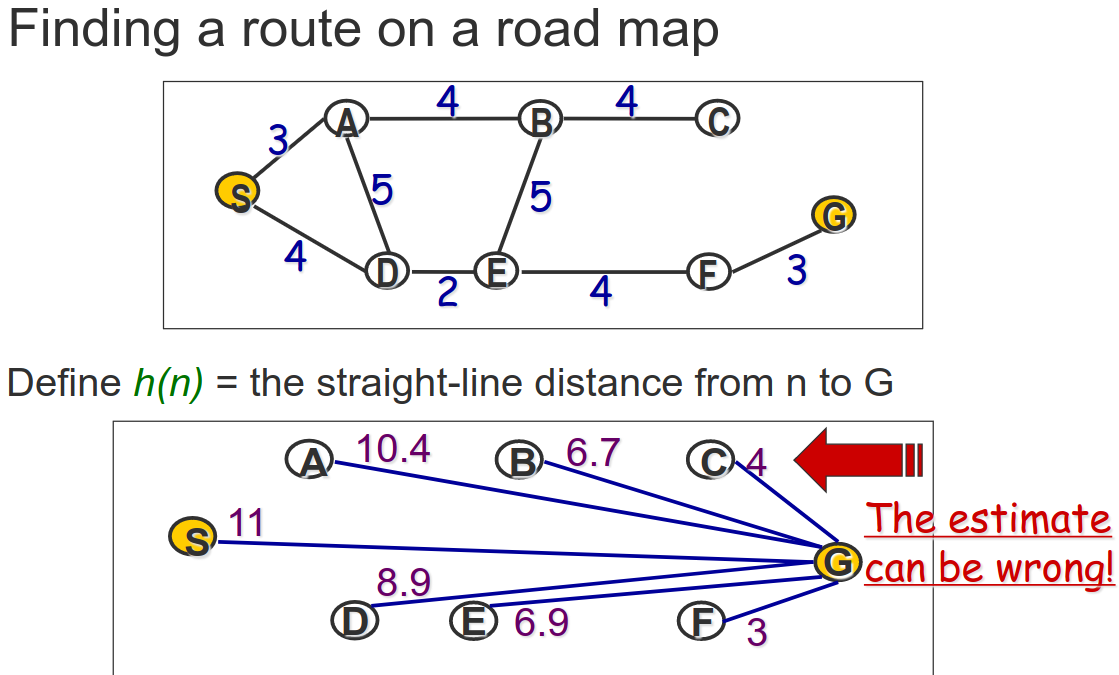
\includegraphics[width=0.8\textwidth]{img/ExempleHeuristic.png}

		\end{figure}
		
		Il y a 3 types de fonction Heuristique :
		\begin{itemize}
			\item \textbf{Optimistic} : Admissible car elle pense que le cout pour résoudre le problème est inférieur au cout réel
			\item \textbf{Admissible} : Ne surestime jamais le cout pour atteindre le goal. Le cout qu'il estime est plus grand que le plus petit cout possible par rapport au node actuel. $h(n) = 0$ si c'est un Goal state.
			\item \textbf{Consistent} : L'estimation de un node $n$ au goal est plus petit que le cout réel de $n$ a un nouveau node $n'$ avec l'action $a$ plus l'estimation de $n'$ au goal 
			\begin{equation}
				h(n) \leq c(n,a,n') + h(n')
			\end{equation}
		\end{itemize}
		
		un consistent heuristi est admissible
		
		\subsubsection{Triangle inequality}
			\begin{figure}[htp]
				\centering
				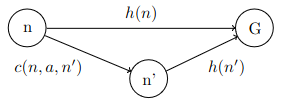
\includegraphics[scale=1]{img/Triangle.png}
			\end{figure}
			Chaque coté du triangle ne peut pas être plus long que la somme des autres cotés.
			\begin{itemize}
				\item \textbf{h(n)} : Estime le cout entre $n$ et $G$
				\item \textbf{C(n,a,n')} : cout pour aller en $n'$ depuis $n$ avec l'action $a$
				\item \textbf{h(n')} : cout estimé entre $n'$ et $G$
			\end{itemize}
			
		\subsubsection{Monotonicity} 
			Si $h(n)$ est consistant alors f(n) le long d'un path quelconque n'est pas décroissant. Supposons que $n'$ est un successeur de $n$ alors :
			
			\begin{figure}[htp]
				\centering
				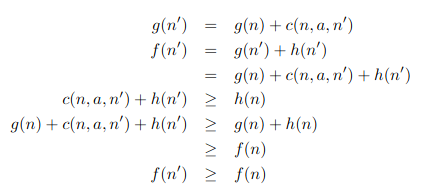
\includegraphics[scale=1]{img/Monotonicité.png}
			\end{figure}
		\subsubsection{Greedy Best-First Search(GBFS)}
			Tente d'étendre le node qui est le plus proche du Goal.
			
			Attention il n'est pas optimal et pas complet car il peut loop
			
			Sa \textbf{Time compexity} et \textbf{Space complexity} est $\mathcal{O}(b^m)$
			
			\begin{figure}[htp]
				\centering
				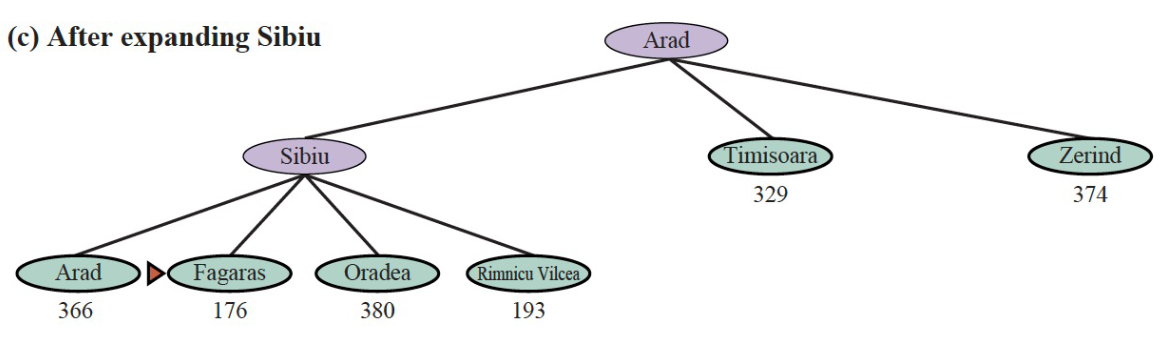
\includegraphics[width=\textwidth]{img/GBFS.png}
			\end{figure}
		\subsubsection{A*}
		Fusion de GBFS et Uniform cost. Minimise le cout total estimé de la solution
		
		\begin{figure}[H]
			\centering
			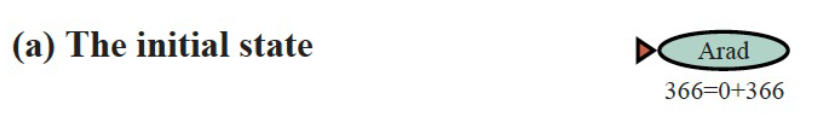
\includegraphics[width=\textwidth]{img/A.png}
		\end{figure}
		\begin{figure}[H]
			\centering
			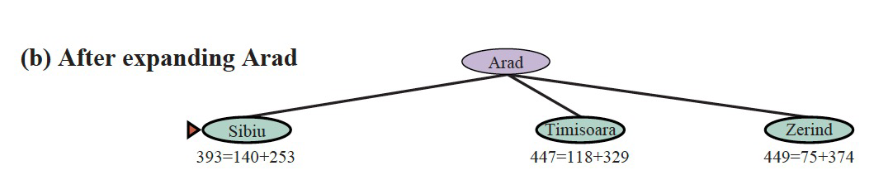
\includegraphics[width=\textwidth]{img/A1.png}
		\end{figure}\begin{figure}[H]
			\centering
			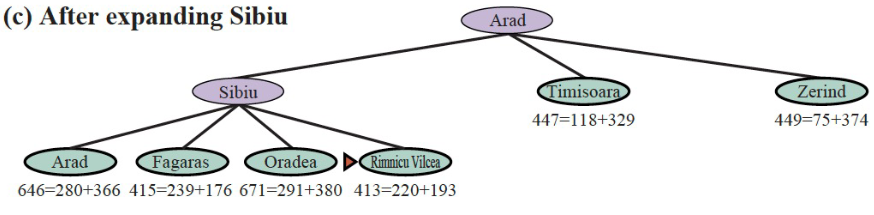
\includegraphics[width=\textwidth]{img/A2.png}
		\end{figure}\begin{figure}[H]
			\centering
			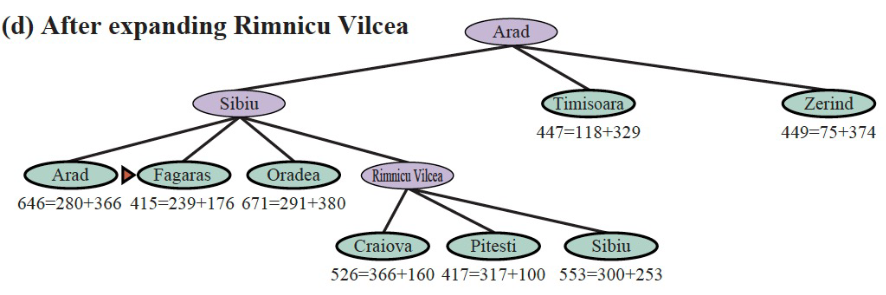
\includegraphics[width=\textwidth]{img/A3.png}
		\end{figure}\begin{figure}[H]
			\centering
			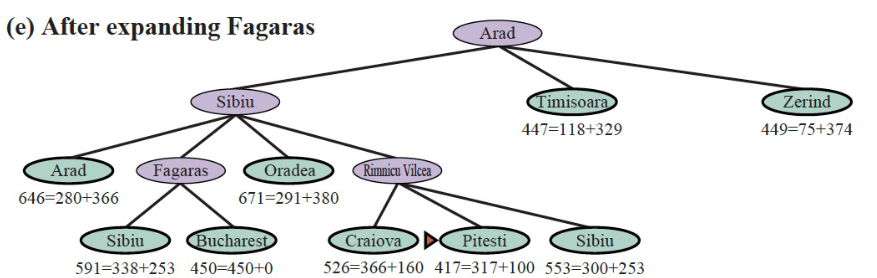
\includegraphics[width=\textwidth]{img/A4.png}
		\end{figure}\begin{figure}[H]
			\centering
			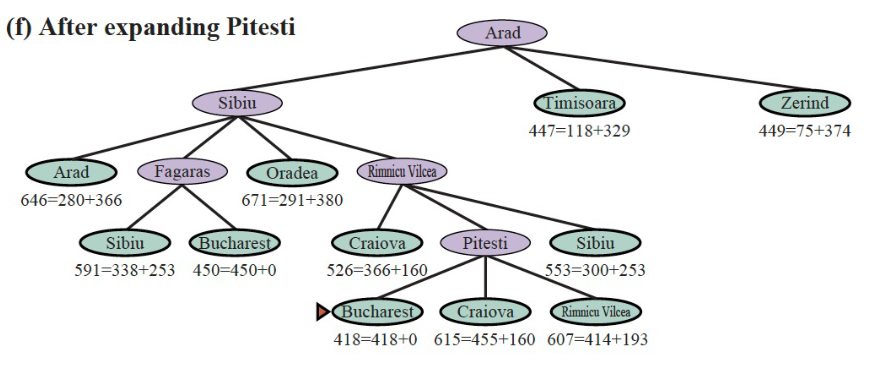
\includegraphics[width=\textwidth]{img/A5.png}
		\end{figure}
		
		A* utilise la distance et additionne la distance actuelle vers le goal. $g(n)$ le cout de la solution vers le node n et $h(n)$ la fonction heuristique
		\begin{equation}
			f(n) = g(n) + h(n)
		\end{equation}
		
		$h(n)$ ne doit pas surestimer le cout vers le goal
		
		\textbf{Time et Space complexity} = $\mathcal{O}(b^d)$ un bon algo mais prend trop de mémoire.
		
		L'algo est \textbf{Complete} si le cout ne peut pas être négatif, il est \textbf{optimal} si la fonction heuristique est admissible (tree) ou consistent(graph)
			
			
		Propriété de A* :
		\begin{itemize}
			\item Avec $h(n)$ consistent, la séquence de nodes étendues par $A*$  est pas d'ordre décroissance de$f(n)$
			\item A* est optimal si $h(n)$ est consistent
			\item A* étend tous les nodes avec $f(n) \leq C^*$ ($C^*$ est le cout optimal)
			\item A* étend au moins un node du contour de $C^*$ avant de le trouver
			\item A* étend aucun node avec $f(n) > C^*$
		\end{itemize}
		
		Pour la preuve que A* est optimal $\rightarrow$ Voire slides
		
		\subsubsection{Memory-bounded heuristic search}
		On tente ici de réduire la mémoire que on a besoin, et on va utiliser les fonctions heuristiques pour nous aider.
		
		\textbf{Iterative-deepening A* (IDA*)}
			A* avec une limite de depth $l$ qui est incrémenté itérativement.
			
			IDA* expend seulement les nodes avec f-cost() $\leq$ que les nodes non expand a la dernière itérations.
		
			Ce n'est pas efficace quand le nombre des f-cost() sont élevés.
			
			Propriétés :
			\begin{itemize}
				\item \textbf{Complet}
				\item \textbf{Time complexity} : exponentiel
				\item \textbf{Space complexity} : Linéaire
				\item \textbf{Optimal et $h()$ consistent}
				\item \textbf{Efficace si absence de monotonicité}
			\end{itemize}
			
		\textbf{Recursive best-first search (RBFS)}
			Pareil que DFS mais ne va pas au bous de la branche, mais utilise $f_{limit}$  pour garder la trace de la valeur f-value du meilleur chemin alternatif a partir de l'ancêtre du node actuel.
			
			\begin{itemize}
				\item \textbf{Time complexity} : Dépend de $h(n)$
				\item \textbf{Space complexity} : $\mathcal{O}(bd)$ si $h(n)$ est admissible
			\end{itemize}
			
			Utilise trop de mémoire
		
		\textbf{SMA*}
			Run avec A* tant que la mémoire est pas pleine. Quand elle est plaine, on doit supprimer un node pour le remplacer, on va donc retirer le pire node (avec la plus grande valeur f-value)
		
		Propriétés :
			\begin{itemize}
				\item \textbf{Complet} si assez de mémoire pour le path de la solutions la plus courte
				\item \textbf{Optimal} si assez de mémoire pour enregistrer le path de la meilleur solutions
				\item \textbf{Time complexity} : Pareil que A* si assez de mémoire pour le tree
				\item \textbf{Space complexity} : utilise ce qui est disponible
			\end{itemize}
		
	
	\subsection{Heuristic en pratique}
		On doit utiliser un heuristique \textbf{Admissible} et \textbf{Consistent}.
		
		Pour comparer 2 heuristique, il faut comparer :
		\begin{itemize}
			\item le nombre de nodes genérées
			\item le facteur de branchage $b^*$
		\end{itemize}
		